\chapter{Volume, Trust, and the Hard Questions of Sales}

This chapter records an entrepreneurship interview from School of Hard Knocks, curated by LazyingArt LLC with Video2Book, as a case study in early sales judgment. The central speaker is Jacob Hopkins, introduced as a nineteen-year-old college dropout who moved from more than \(\$10{,}000\) in debt to more than \(\$250{,}000\) per year in sales. The point is not to turn one interview into a universal formula. The point is to preserve the operating logic that the conversation unfolds: volume reduces dependence on luck, listening precedes persuasion, challenge replaces empty agreement, and hard questions are part of commercial care.

\section{The Opening Case}

James opens by naming the context: he and Josh are visiting Jacob Hopkins to extract practical sales lessons for someone starting out. The opening claim is quantitative and should stay quantitative:

\begin{equation}
D > \$10{,}000,
\qquad
I_{\mathrm{sales}} > \$250{,}000/\mathrm{year}.
\end{equation}

Here \(D\) is the debt level reported in the introduction, and \(I_{\mathrm{sales}}\) is the reported annual sales income. These are interview claims, not audited statements, but they do useful work in the lecture: they establish why Jacob's later advice is not merely attitude. It is tied to a before-and-after commercial path.

Before Jacob gives the five sales tips, the interview briefly passes through Quinn Fulmer, who works on YouTube content at acquisition.com. Quinn's advice to content creators is that short form can get people in the door, but fast imitation is a poor foundation. He puts the creator's path on a three-, five-, or ten-year horizon. That aside matters because it introduces the chapter's first recurring principle: a short-term tactic only becomes valuable when it serves a long-term identity and skill path.

\section{Searching For The Skill}

Jacob's own story begins with restless business searching. In high school he was business minded, did not want an ordinary path, and tried several vehicles: car detailing, dropshipping, and real estate. The early experiments produced a little money, but not a durable engine. The transcript says he made ``a couple grand'' from some attempts, but nothing major.

The important pivot is that he does not describe sales as a passion discovered in the abstract. Sales appears as the skill that could make the rest of his entrepreneurial ambition operational. Pepperdine, in his telling, became the institution around which the sales opportunity opened, and two years later he says he has not looked back.

This gives the first structural lesson of the interview. The sequence is not

\begin{equation}
\hbox{dream} \longrightarrow \hbox{business} \longrightarrow \hbox{money}.
\end{equation}

It is closer to

\begin{equation}
\hbox{experiments} \longrightarrow \hbox{missing skill} \longrightarrow \hbox{sales repetition} \longrightarrow \hbox{income}.
\end{equation}

The chapter should preserve this order. Jacob does not begin with a framework. He begins with pressure, failed or partial attempts, and then the need for a skill that could compound.

\section{Volume Negates Luck}

When the interview formally asks for the five best tips for someone starting in sales, Jacob's first answer is direct: volume negates luck. He grounds the claim in his real estate period. He says he was losing three or four thousand dollars per month, and was told that the reason was that he was weak at sales.

The monthly loss is the pressure variable:

\begin{equation}
L \approx \$3{,}000\hbox{--}\$4{,}000/\mathrm{month}.
\end{equation}

The prescription was not subtle: if everyone else is making \(100\) calls, make \(200\). Jacob reports making \(200\), \(300\), and \(400\) dials per day while others were around \(100\):

\begin{equation}
N_{\mathrm{others}} \approx 100 \ \mathrm{calls/day},
\qquad
N_{\mathrm{Jacob}} \approx 200\hbox{--}400 \ \mathrm{dials/day}.
\end{equation}

A cautious way to model the claim is to let \(N\) be qualified sales attempts and \(p\) be the probability that one attempt eventually closes. The interview does not give \(p\), so this is only a reconstruction of the mechanism:

\begin{equation}
\mathbb{E}[\hbox{closed deals}] \approx Np.
\end{equation}

If \(p\) were fixed, doubling \(N\) doubles the expected number of opportunities:

\begin{equation}
\frac{\mathbb{E}[\hbox{deals}_{200}]}{\mathbb{E}[\hbox{deals}_{100}]}
\approx
\frac{200p}{100p}
=
2.
\end{equation}

That equation is not a promise. It is the cleanest mathematical version of Jacob's point: a beginner has limited control over charisma, timing, or the mood of any one prospect, but does have control over the number of honest repetitions. Jacob says that within two or three weeks he was doing about as well as the others because he was putting up more numbers.

\subsection{Question \& Answer}

\paragraph{Question.}
If sales outcomes feel random, what can a beginner actually control?

\paragraph{Answer.}
The beginner controls the number of attempts and the seriousness of each repetition. The lecture's claim is not that volume makes skill unnecessary. It is that volume gives skill enough trials to form. If a single call is noisy, then the day's activity is the more meaningful unit of work.

\begin{figure}
\centering
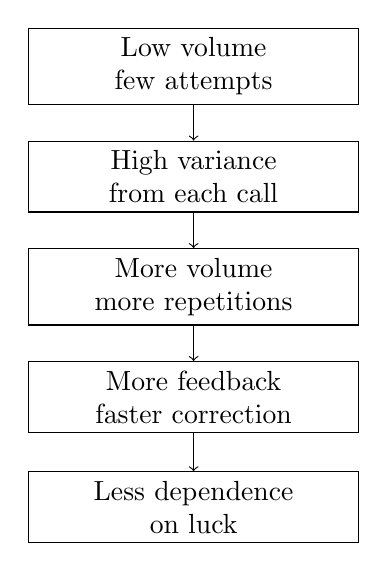
\begin{tikzpicture}[x=1cm,y=1cm]
\node[draw, align=center, minimum width=4.2cm, minimum height=0.7cm] (a) at (0,0) {Low volume\\few attempts};
\node[draw, align=center, minimum width=4.2cm, minimum height=0.7cm] (b) at (0,-1.4) {High variance\\from each call};
\node[draw, align=center, minimum width=4.2cm, minimum height=0.7cm] (c) at (0,-2.8) {More volume\\more repetitions};
\node[draw, align=center, minimum width=4.2cm, minimum height=0.7cm] (d) at (0,-4.2) {More feedback\\faster correction};
\node[draw, align=center, minimum width=4.2cm, minimum height=0.7cm] (e) at (0,-5.6) {Less dependence\\on luck};
\draw[->] (a) -- (b);
\draw[->] (b) -- (c);
\draw[->] (c) -- (d);
\draw[->] (d) -- (e);
\end{tikzpicture}
\caption{A pocket-size reconstruction of the lecture's first sales mechanism: volume turns isolated luck into repeated feedback.}
\end{figure}

\section{Performance Means Health Plus Action}

The interviewer next presses on the cost of that advice. Sales is a high-performance job. If the prescription is more calls, then the obvious question is how to remain able to make them.

Jacob's answer has two parts. First, he names health: sleep and basic care of the body. Second, he names action as the antidote to stress. He says the biggest cause of stress for him is inaction. If he is not hitting the phones or doing what he knows he needs to do, he gets stressed.

The relation is best kept as prose, not as a fake psychological formula. Still, the operating distinction is precise:

\begin{equation}
\hbox{focus on result} \quad \hbox{is replaced by} \quad \hbox{focus on daily action}.
\end{equation}

The business reason is simple. A result may arrive late, or arrive after several failed attempts. Action is the unit one can schedule, repeat, inspect, and improve.

\subsection{Question \& Answer}

\paragraph{Question.}
How does someone maintain high performance without becoming trapped by the outcome?

\paragraph{Answer.}
Jacob's answer is to move attention from the result to the action. Sleep and health keep the system capable. Daily activity keeps the mind from converting uncertainty into stress. In the chapter's language, the result is the lagging variable; action is the controllable input.

\section{Listen More, Pitch Less}

The second sales tip is ``listen more, talk less.'' Jacob pushes against the novice picture of sales as a talking job. A salesperson must be articulate, but the sale is not won by filling the room with words. It is won by understanding what the buyer needs, wants, fears, and is trying to accomplish.

The pitch then becomes short because it is no longer generic. Jacob says his pitch is less than a minute:

\begin{equation}
T_{\mathrm{pitch}} < 1\ \mathrm{minute}.
\end{equation}

The preceding listening does the work. In a compact process notation:

\begin{equation}
\hbox{questions}
\longrightarrow
\hbox{diagnosis}
\longrightarrow
\hbox{trust}
\longrightarrow
\hbox{short pitch}
\longrightarrow
\hbox{ask}.
\end{equation}

This is a useful place to separate anecdote, claim, and mechanism. The anecdote is Jacob saying that good questions can make the prospect ready before the pitch begins. The claim is that active listening builds trust and rapport. The mechanism is that the salesperson can then present only the relevant three things rather than dumping every feature into the conversation.

\section{The Long Horizon And The Right Challenge}

The interview then asks Jacob what he would tell his younger self. This reflective question is not a break from the sales tips; it is the bridge into the next one. Jacob says he would keep betting on himself and think over a long time horizon. He contrasts trying to become a millionaire in \(90\) days with thinking in \(10\) years:

\begin{equation}
T_{\mathrm{fantasy}} \approx 90\ \mathrm{days},
\qquad
T_{\mathrm{skill}} \approx 10\ \mathrm{years}.
\end{equation}

The garbled transcript around this point appears to be about stacking skill sets, especially learning sales if one's future business requires selling. The safe reconstruction is modest: choose the skill that aligns with the ten-year path.

That leads directly into sales tip number three: challenge people. Jacob distinguishes challenge from hostility. In his framing, the salesperson is not the prospect's casual friend, but also not an enemy. The salesperson cares enough to test whether the prospect's beliefs and actions match the prospect's stated goals.

\subsection{Question \& Answer}

\paragraph{Question.}
How can a salesperson challenge a prospect without becoming adversarial?

\paragraph{Answer.}
The challenge has to be tied to the prospect's own stated goal. Jacob's example is a gym owner who wants to double membership in two years while relying on word of mouth. The salesperson does not attack the person. The salesperson tests the plan: will that method really produce the desired number of members?

The numerical example is the clearest one in the lecture. Jacob asks whether the gym owner expects to gain \(300\) members by word of mouth over two years:

\begin{equation}
\Delta M \approx 300 \ \mathrm{members}
\quad \hbox{over} \quad
T = 2 \ \mathrm{years}.
\end{equation}

As a simple reconstruction, the average burden is

\begin{align}
\frac{\Delta M}{T}
&=
\frac{300 \ \mathrm{members}}{2 \ \mathrm{years}}  \\
&=
150 \ \mathrm{members/year} \\
&\approx
12.5 \ \mathrm{members/month}.
\end{align}

Jacob does not compute the monthly figure in the transcript. But the arithmetic clarifies the challenge: once the target is translated into a required rate, the prospect can see whether the chosen channel is plausible.

\begin{figure}
\centering
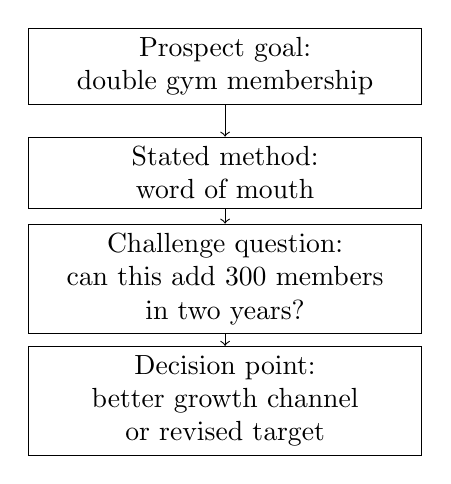
\begin{tikzpicture}[x=1cm,y=1cm]
\node[draw, align=center, minimum width=5.0cm, minimum height=0.7cm] (g) at (0,0) {Prospect goal:\\double gym membership};
\node[draw, align=center, minimum width=5.0cm, minimum height=0.7cm] (m) at (0,-1.35) {Stated method:\\word of mouth};
\node[draw, align=center, minimum width=5.0cm, minimum height=0.7cm] (q) at (0,-2.7) {Challenge question:\\can this add 300 members\\in two years?};
\node[draw, align=center, minimum width=5.0cm, minimum height=0.7cm] (r) at (0,-4.25) {Decision point:\\better growth channel\\or revised target};
\draw[->] (g) -- (m);
\draw[->] (m) -- (q);
\draw[->] (q) -- (r);
\end{tikzpicture}
\caption{Challenge selling as a test of consistency between the prospect's goal and the prospect's method.}
\end{figure}

\section{Commission, Asking, And Referrals}

The next obstacle is risk. New salespeople may be intimidated because many sales roles are primarily commission based. Jacob's answer is not that commission is easy, or that everyone should choose it. His narrower claim is that nothing is truly guaranteed. A salary can disappear if performance is poor. Commission simply makes the performance link more direct.

In that sense, sales is close to ownership. The person manages time, schedule, and output, and gets paid according to production. The compact comparison is

\begin{equation}
\hbox{salary} \approx \hbox{delayed performance risk},
\qquad
\hbox{commission} \approx \hbox{direct performance exposure}.
\end{equation}

The fourth sales tip follows naturally: ask for money. Jacob says too many people in sales do not ask for the order. The sequence is important. He does not say to pitch immediately. He says not to pitch until one knows one can close, and once the pitch is made, actually ask.

He also says he has had people tell him no five or ten times in a row while he continued to solve the problem and ask again:

\begin{equation}
n_{\mathrm{no}} \approx 5\hbox{--}10.
\end{equation}

This is not a license to ignore a prospect's boundaries. In context, the action is to solve the objection or problem and then ask again. The commercial discipline is not mere pressure; it is repeated movement from obstacle to decision.

Networking enters as an extension of the same logic. Jacob describes a sales process where clients see an ad, click, and book a call. After they enter the program, he follows up and asks whether they know anyone else or have referrals. He reports closing two deals in the previous week from that process:

\begin{equation}
R_{\mathrm{closed}} = 2 \ \mathrm{deals/week}
\end{equation}

for that reported week. Again, this is an interview claim, but it is concrete enough to preserve.

\section{Stress And Hard Questions}

Near the end, the interviewer returns to beginner stress. Jacob first normalizes it. Stress can appear even when one is doing well because the next thing remains uncertain. His first step is to register stress as a feeling rather than as a command.

His second step is action: put in more work, watch more game tape, listen to more sales calls, and do what can be done. The causal claim is plain: the more useful action he takes, the less idle room there is for stress.

The fifth tip is that closers ask hard questions. Jacob names examples: how much money is in the prospect's bank account, what happens if the problem is not fixed, what life looks like in five years without a solution, and what it looks like if the desired outcome happens.

\subsection{Question \& Answer}

\paragraph{Question.}
Why should a salesperson ask questions that feel awkward?

\paragraph{Answer.}
Because the salesperson cannot responsibly recommend a program without knowing whether the prospect can succeed in it. Jacob says he cannot sign someone into the program if they do not have enough money to be successful. The hard question is therefore not decoration. It is part of diagnosis.

The final mechanism of the chapter can be written as a compact loop:

\begin{figure}
\centering
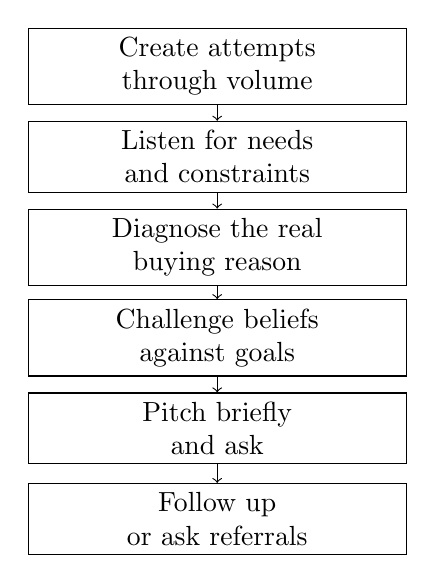
\begin{tikzpicture}[x=1cm,y=1cm]
\node[draw, align=center, minimum width=4.8cm, minimum height=0.65cm] (a) at (0,0) {Create attempts\\through volume};
\node[draw, align=center, minimum width=4.8cm, minimum height=0.65cm] (b) at (0,-1.15) {Listen for needs\\and constraints};
\node[draw, align=center, minimum width=4.8cm, minimum height=0.65cm] (c) at (0,-2.3) {Diagnose the real\\buying reason};
\node[draw, align=center, minimum width=4.8cm, minimum height=0.65cm] (d) at (0,-3.45) {Challenge beliefs\\against goals};
\node[draw, align=center, minimum width=4.8cm, minimum height=0.65cm] (e) at (0,-4.6) {Pitch briefly\\and ask};
\node[draw, align=center, minimum width=4.8cm, minimum height=0.65cm] (f) at (0,-5.75) {Follow up\\or ask referrals};
\draw[->] (a) -- (b);
\draw[->] (b) -- (c);
\draw[->] (c) -- (d);
\draw[->] (d) -- (e);
\draw[->] (e) -- (f);
\end{tikzpicture}
\caption{The sales control loop reconstructed from Jacob Hopkins's five tips.}
\end{figure}

\section{Summary}

The interview's structure is simple but not shallow. It begins with a young seller's reported transformation, passes through early experiments and long-horizon thinking, and then distills five operating rules. Volume gives the beginner repetitions. Health and action sustain performance. Listening makes the pitch short. Challenge tests whether the prospect's method matches the prospect's goal. Commission exposes the seller to performance, asking for the order turns diagnosis into decision, and hard questions make the close responsible rather than merely agreeable.

The mathematical content is modest because the source is not a chalkboard lecture. But the arithmetic is still useful. The chapter keeps the quantities that make the advice concrete: \(\$10{,}000\) in debt, \(\$250{,}000\) per year in reported sales income, \(\$3{,}000\) to \(\$4{,}000\) in monthly losses, \(100\) calls versus \(200\) to \(400\) dials per day, a pitch under one minute, \(300\) gym members over two years, five to ten refusals, and two referral deals in a week. Those numbers keep the chapter from drifting into slogans.